\subsection{Signal injection tests} 

\subsubsection{Injection with QCD}


\begin{figure}
\begin{center}
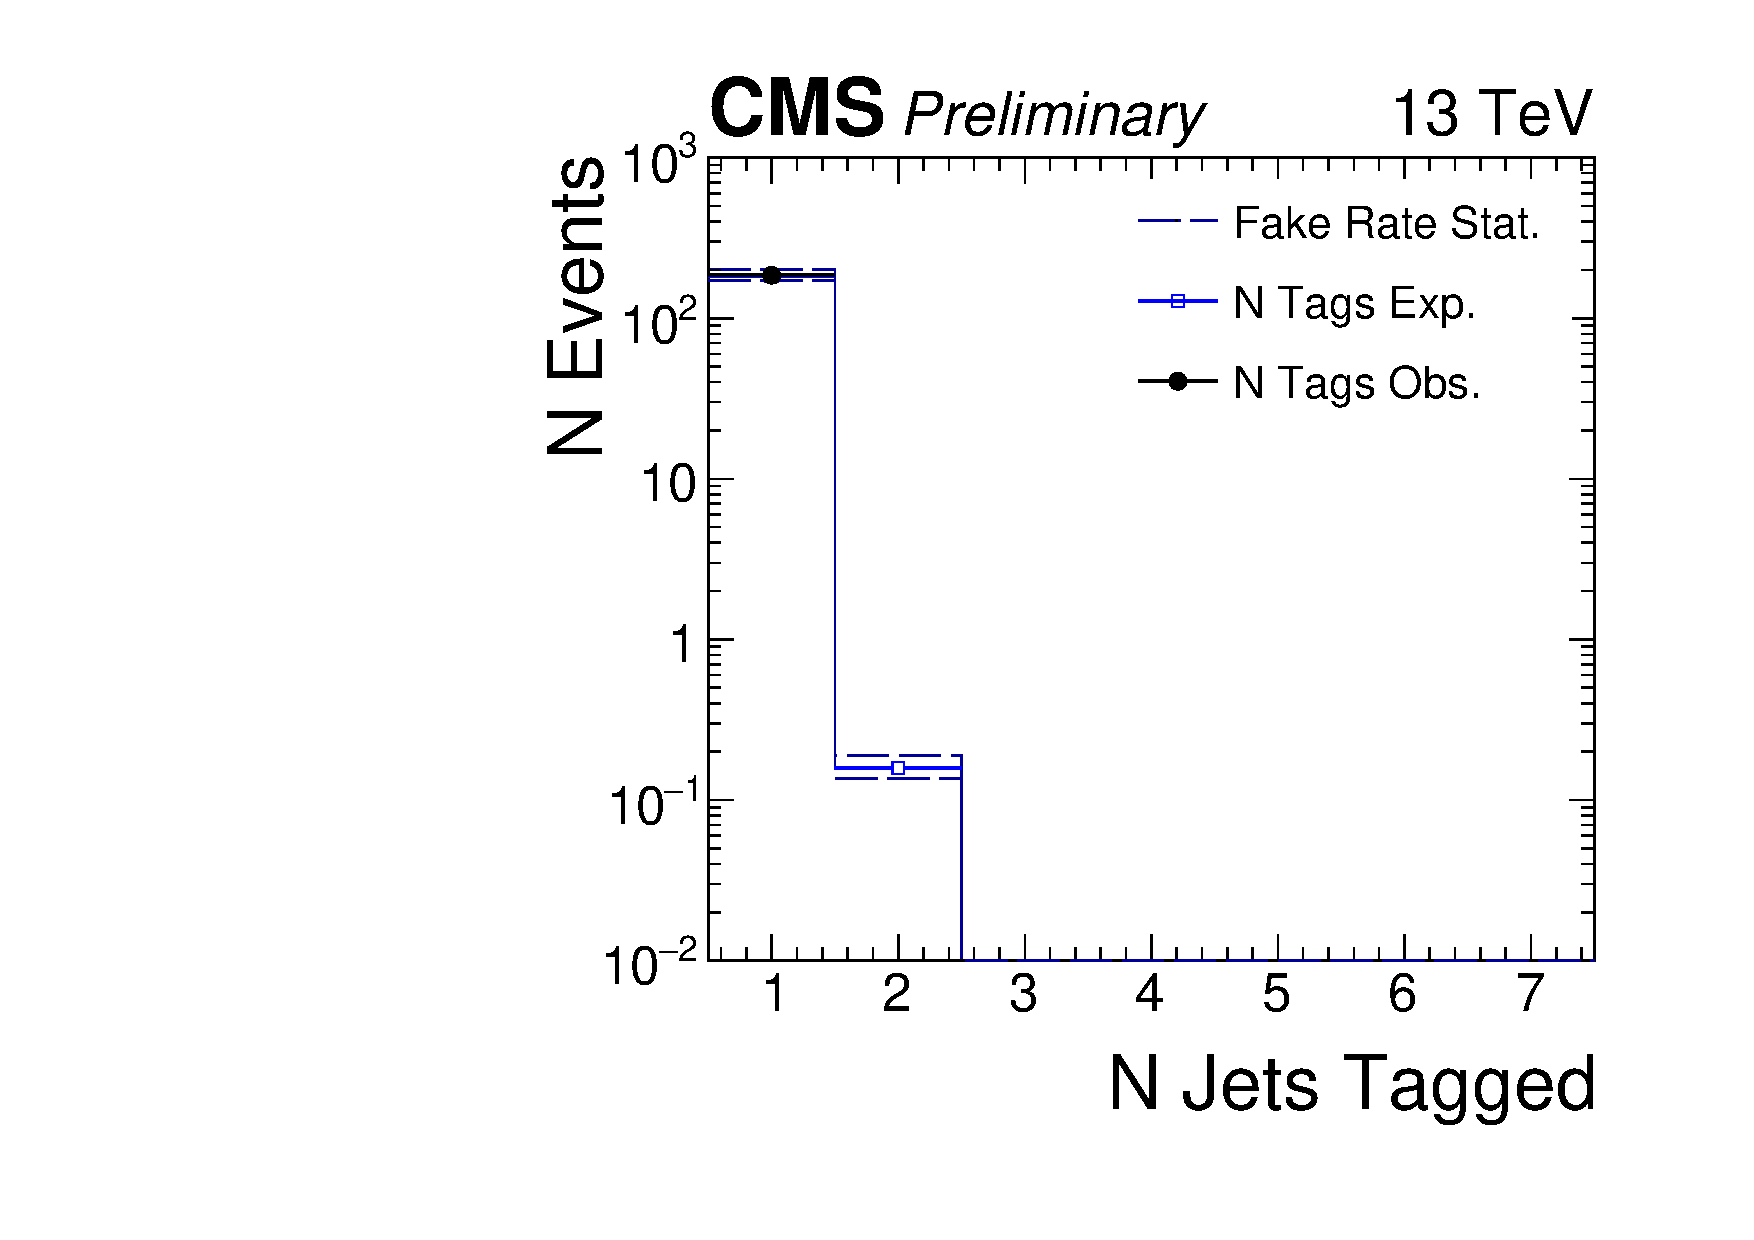
\includegraphics[width=.45\textwidth]{figures/an/ANALYSIS/76x_pu/INJECTION/qcd_loose_displacedEvtSel_0eV.pdf}\\
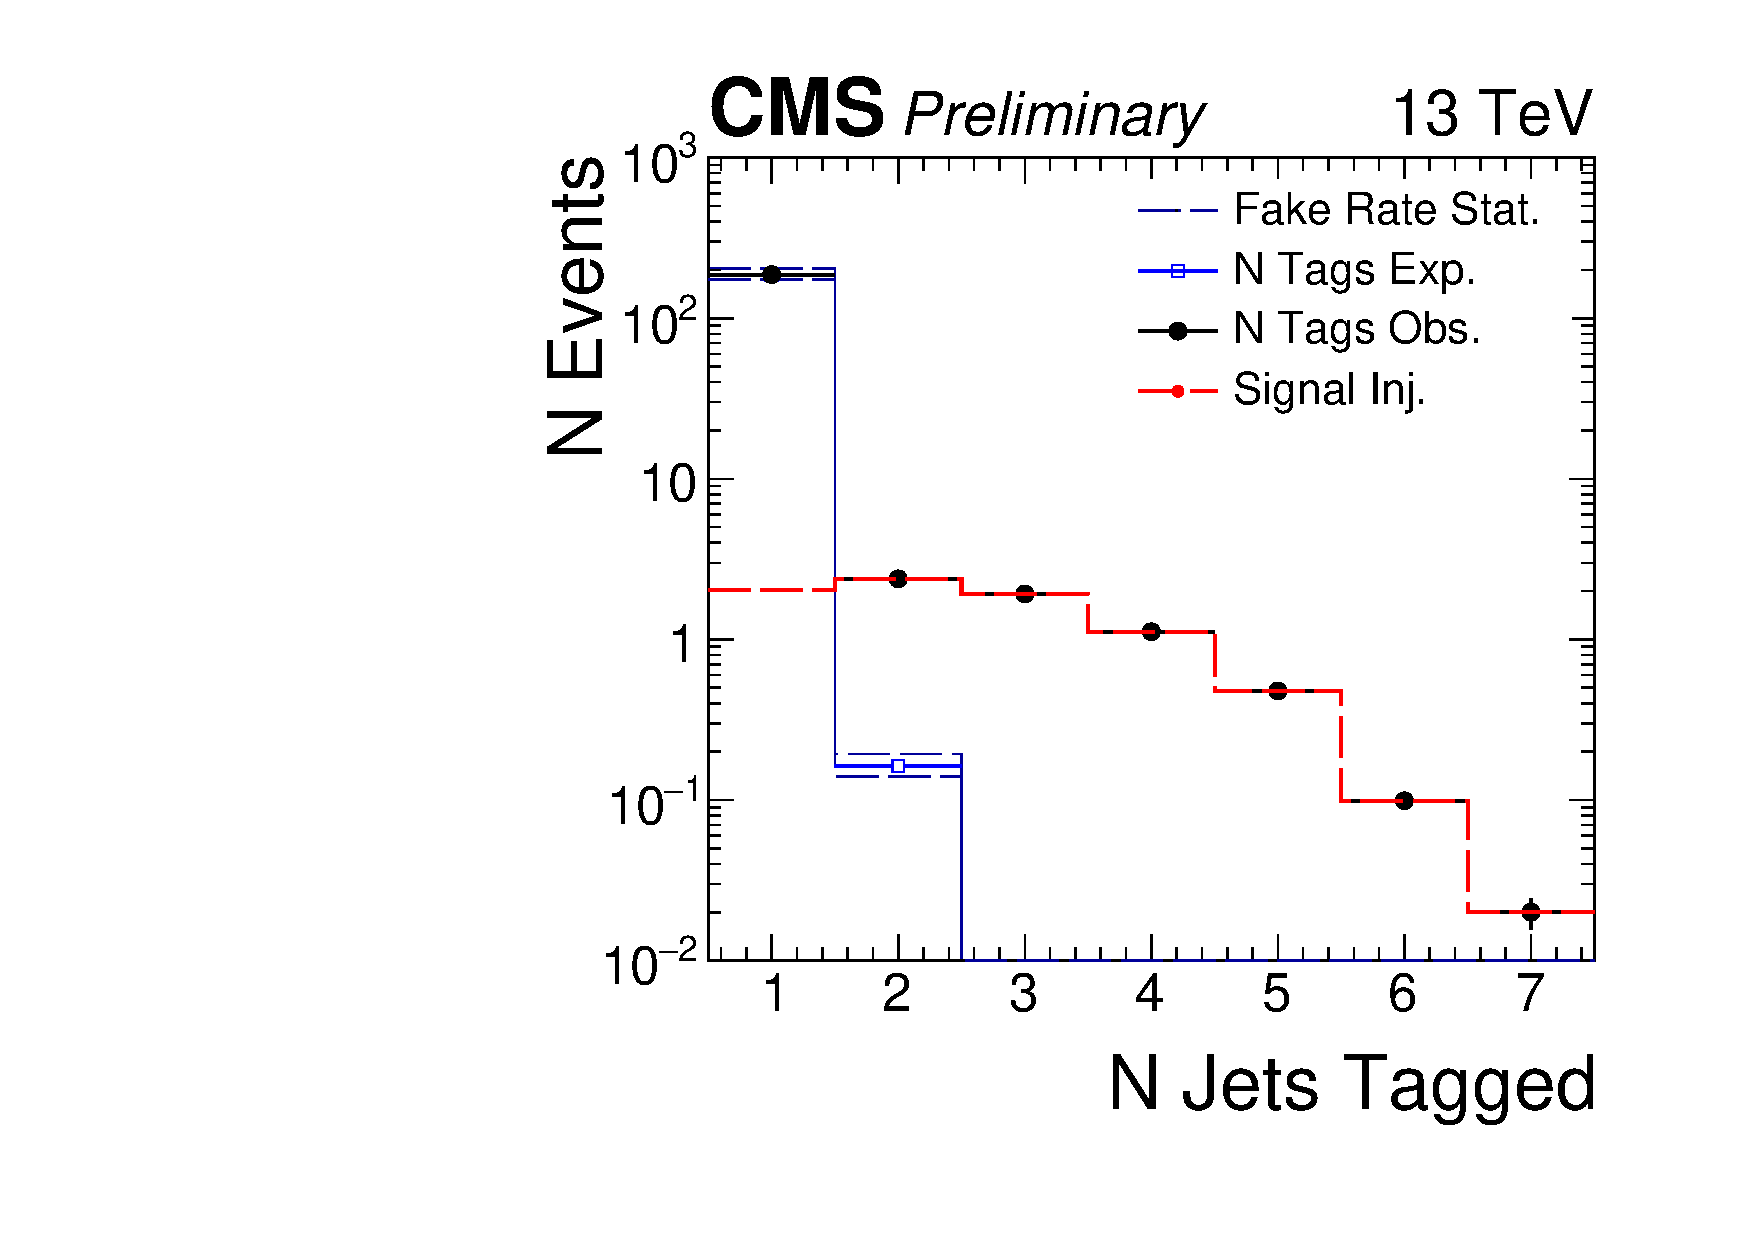
\includegraphics[width=.45\textwidth]{figures/an/ANALYSIS/76x_pu/INJECTION/qcd_loose_displacedEvtSel_10eV.pdf}
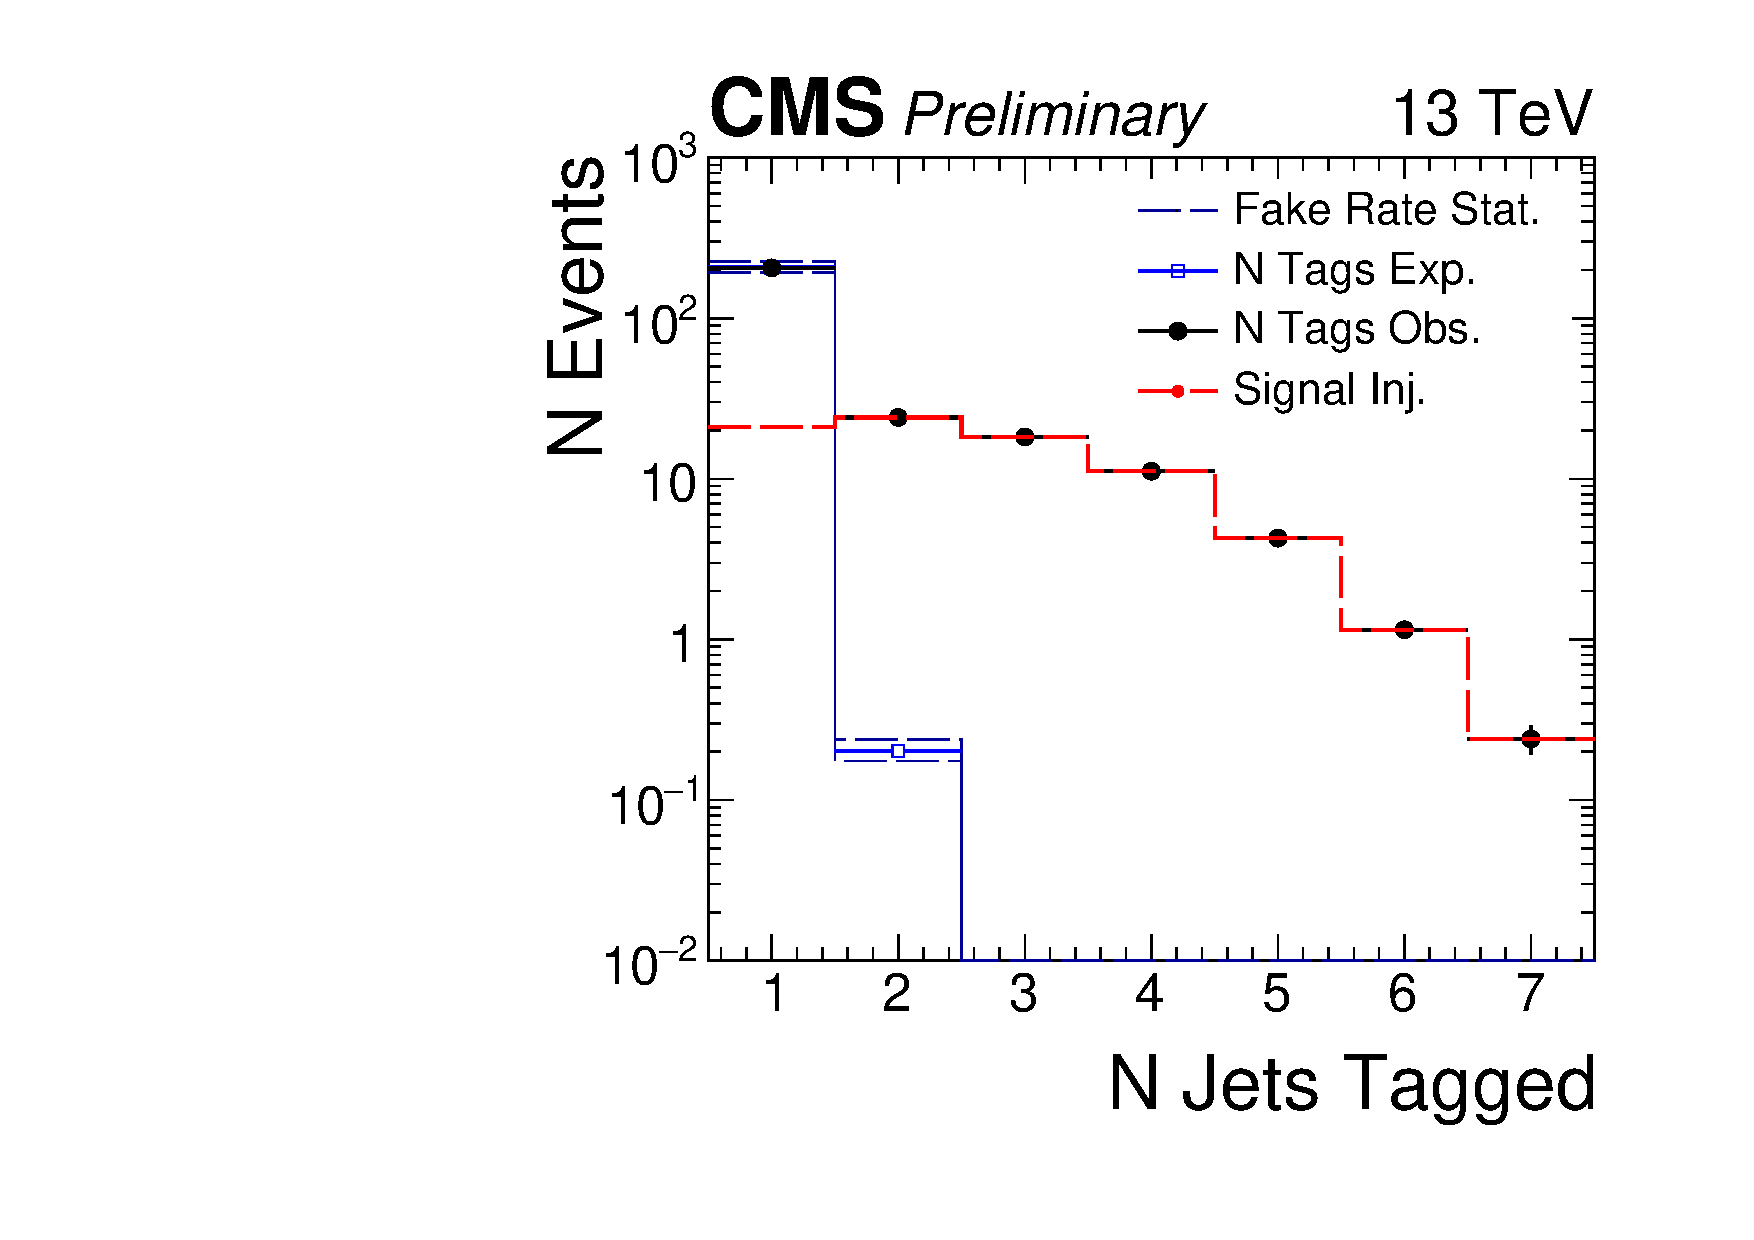
\includegraphics[width=.45\textwidth]{figures/an/ANALYSIS/76x_pu/INJECTION/qcd_loose_displacedEvtSel_100eV.pdf}\\
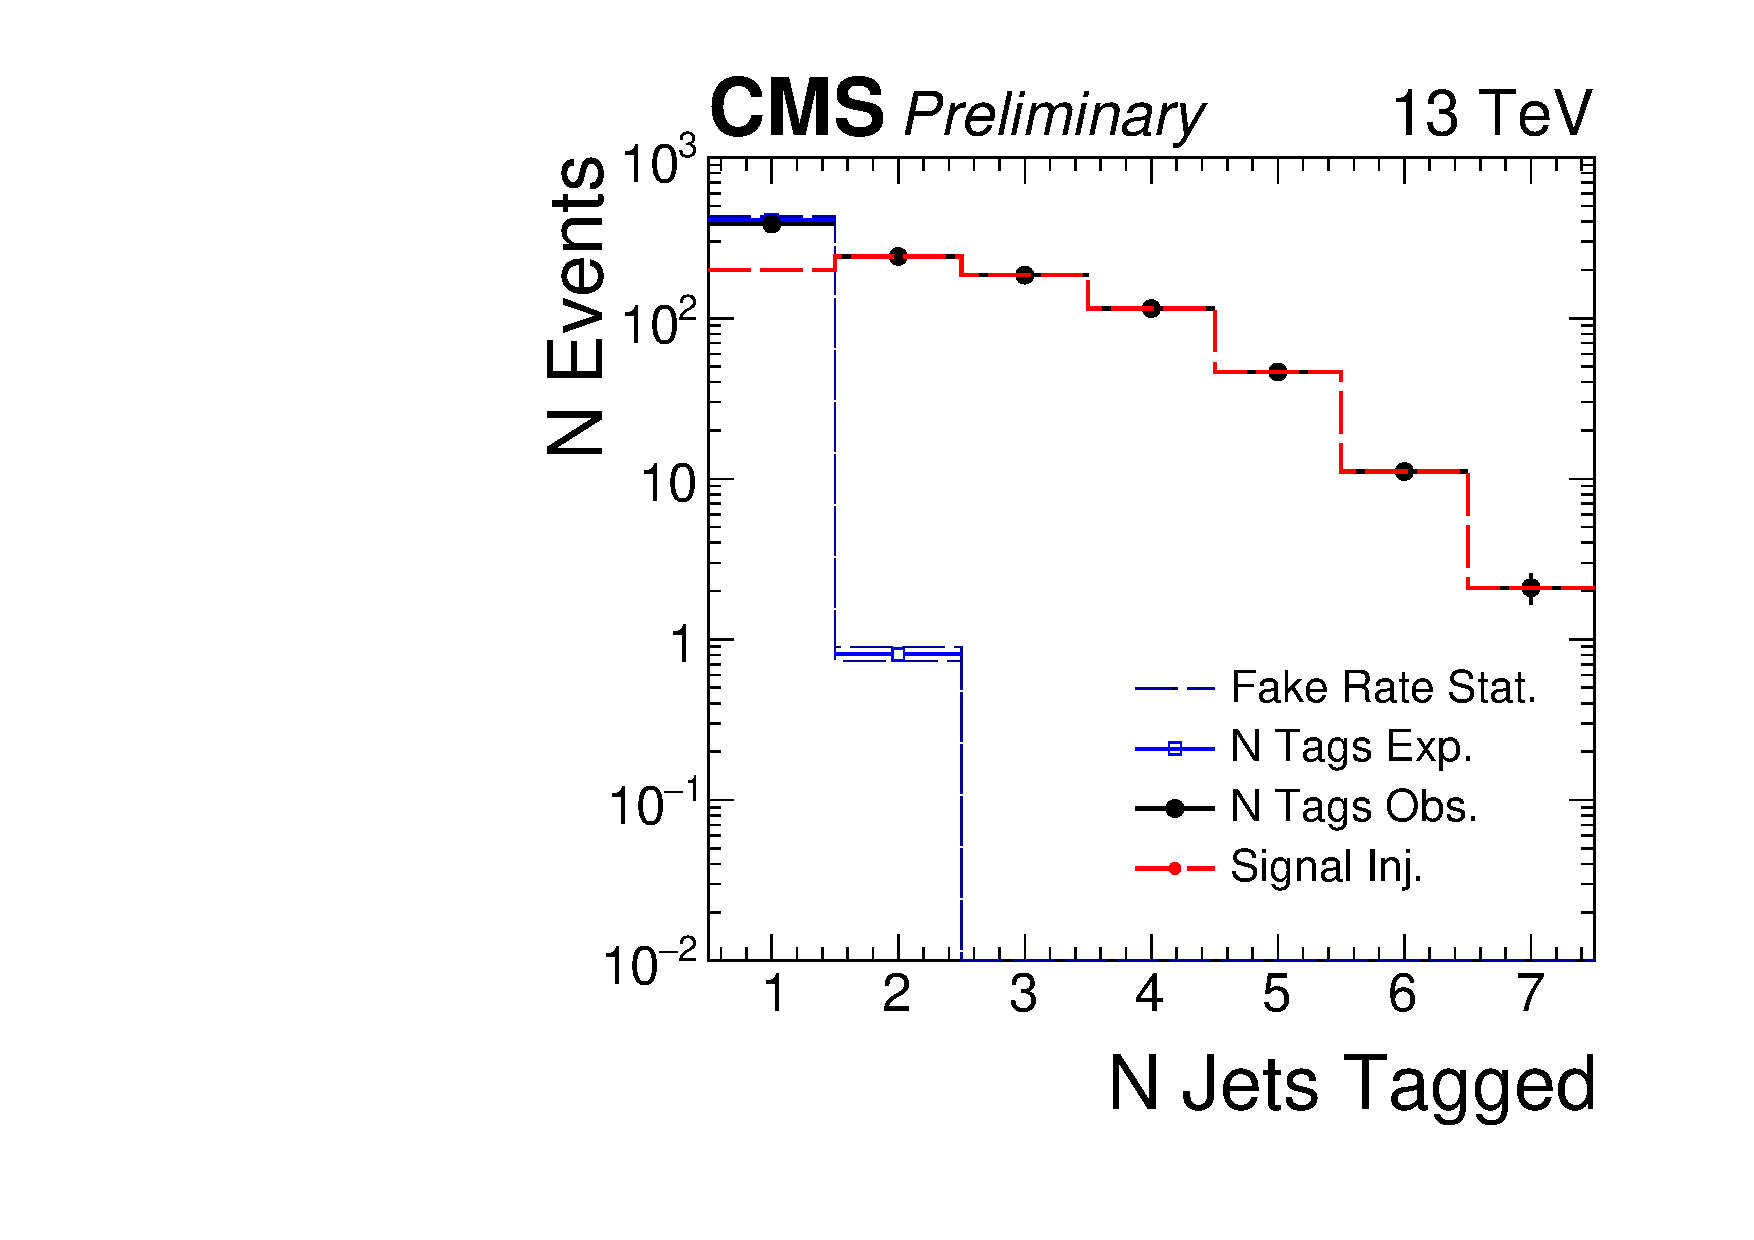
\includegraphics[width=.45\textwidth]{figures/an/ANALYSIS/76x_pu/INJECTION/qcd_loose_displacedEvtSel_1000eV.pdf}
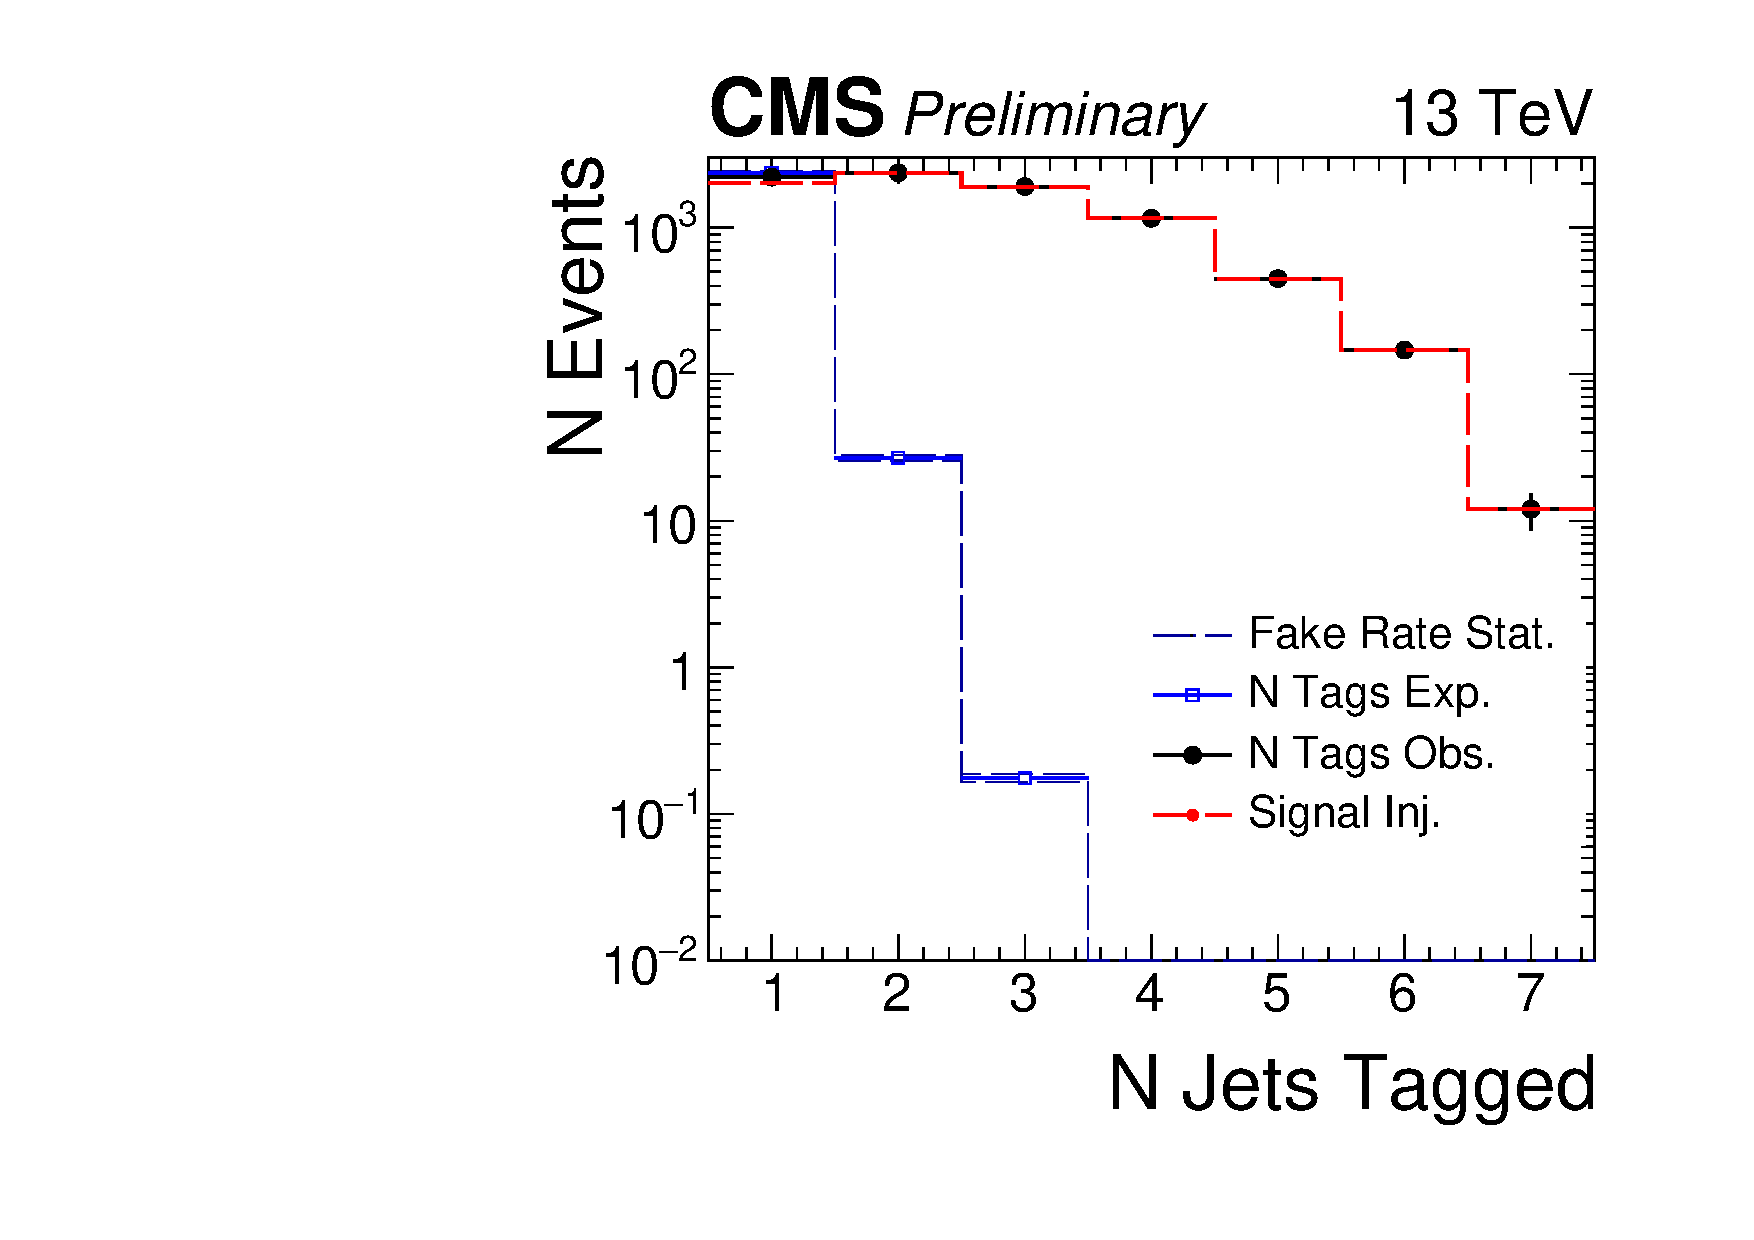
\includegraphics[width=.45\textwidth]{figures/an/ANALYSIS/76x_pu/INJECTION/qcd_loose_displacedEvtSel_10000eV.pdf}
\caption{Signal Injection tests. The Jet-Jet signal sample used has fixed $m_{X^0}=700$ GeV and $c\tau_0=10$ mm. The
level of signal contamination is progressively varied between 10, 100, 1000, and 10000 events injected before any selection. The full 
event selection is applied and the baseline jet tag definition. \label{fig:injection_700_10mm}}
\end{center}
\end{figure}
\begin{figure}
\begin{center}
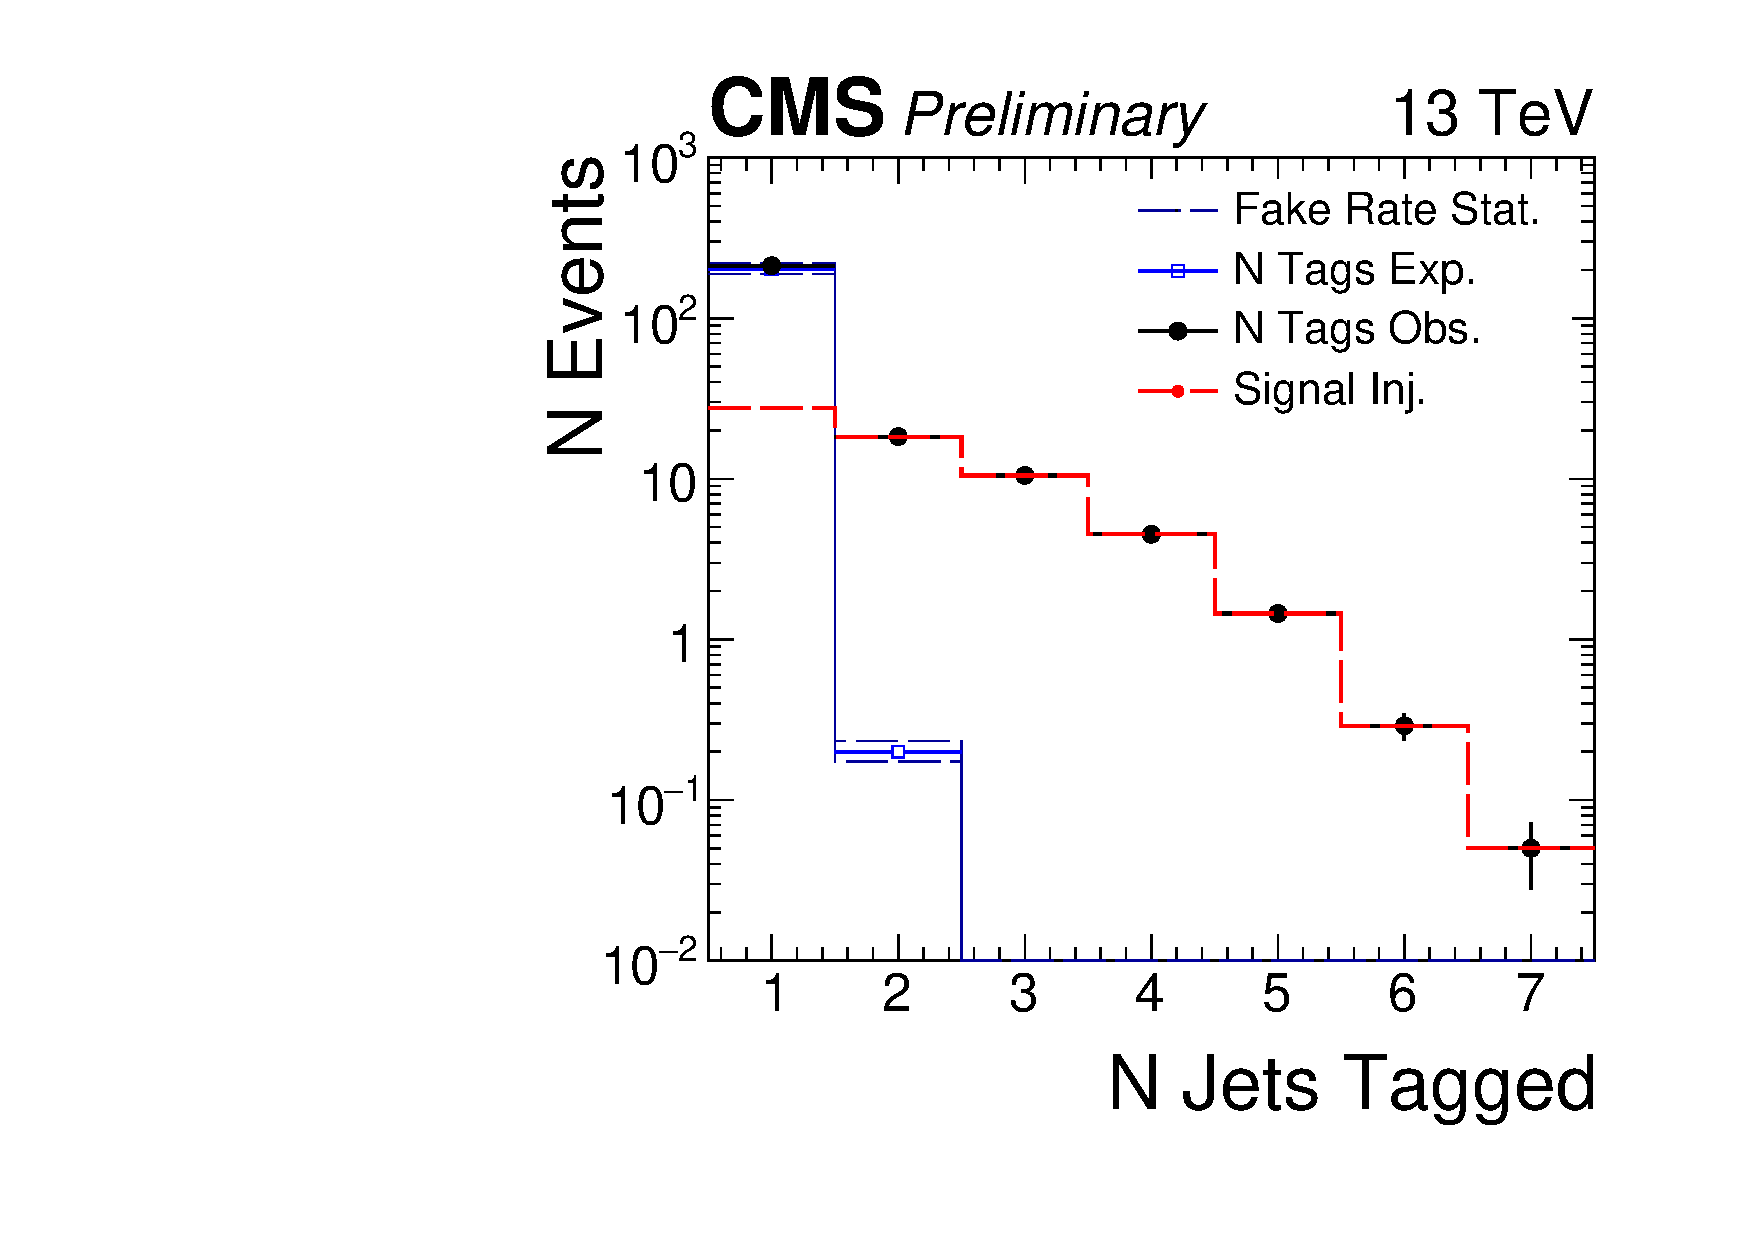
\includegraphics[width=.45\textwidth]{figures/an/ANALYSIS/76x_pu/INJECTION/mx700_ctau1000mm_100ev.pdf}
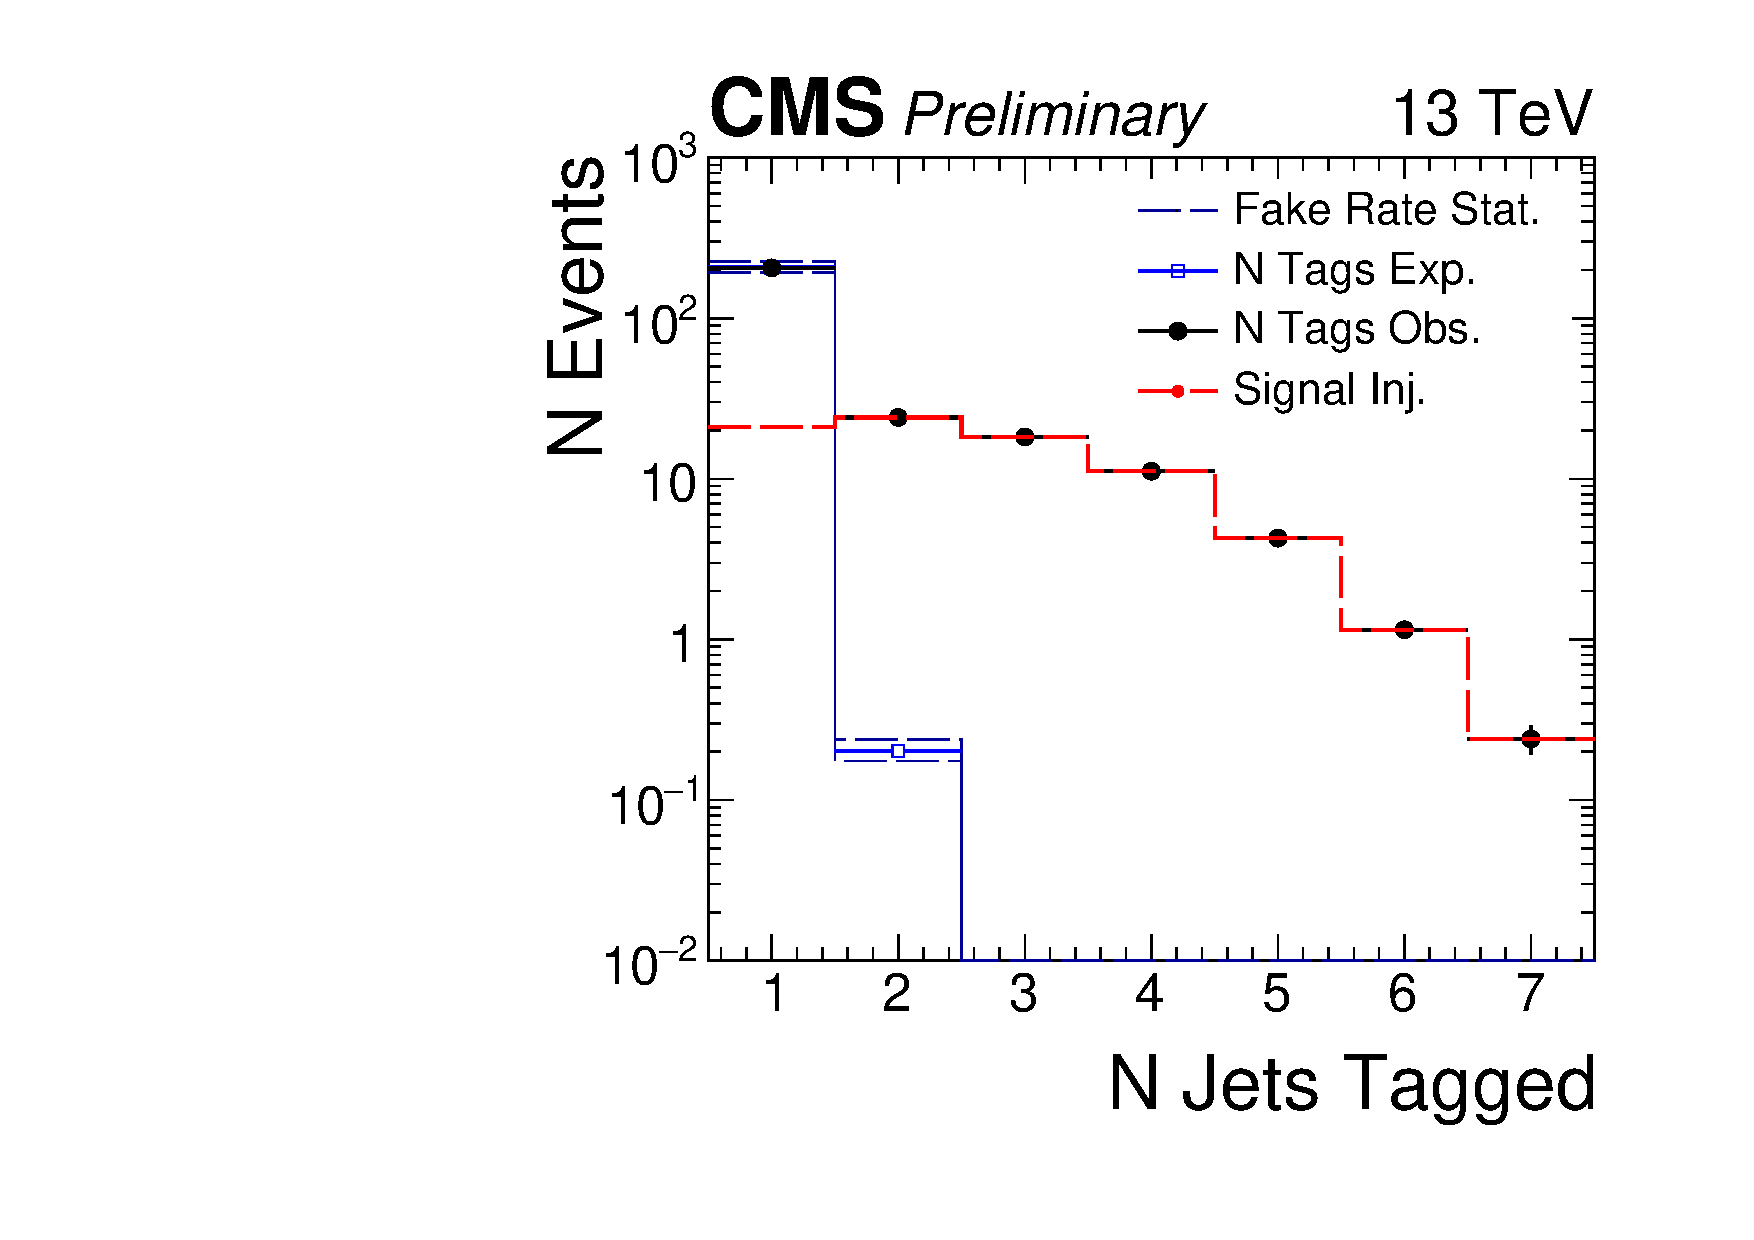
\includegraphics[width=.45\textwidth]{figures/an/ANALYSIS/76x_pu/INJECTION/qcd_loose_displacedEvtSel_100eV.pdf}\\
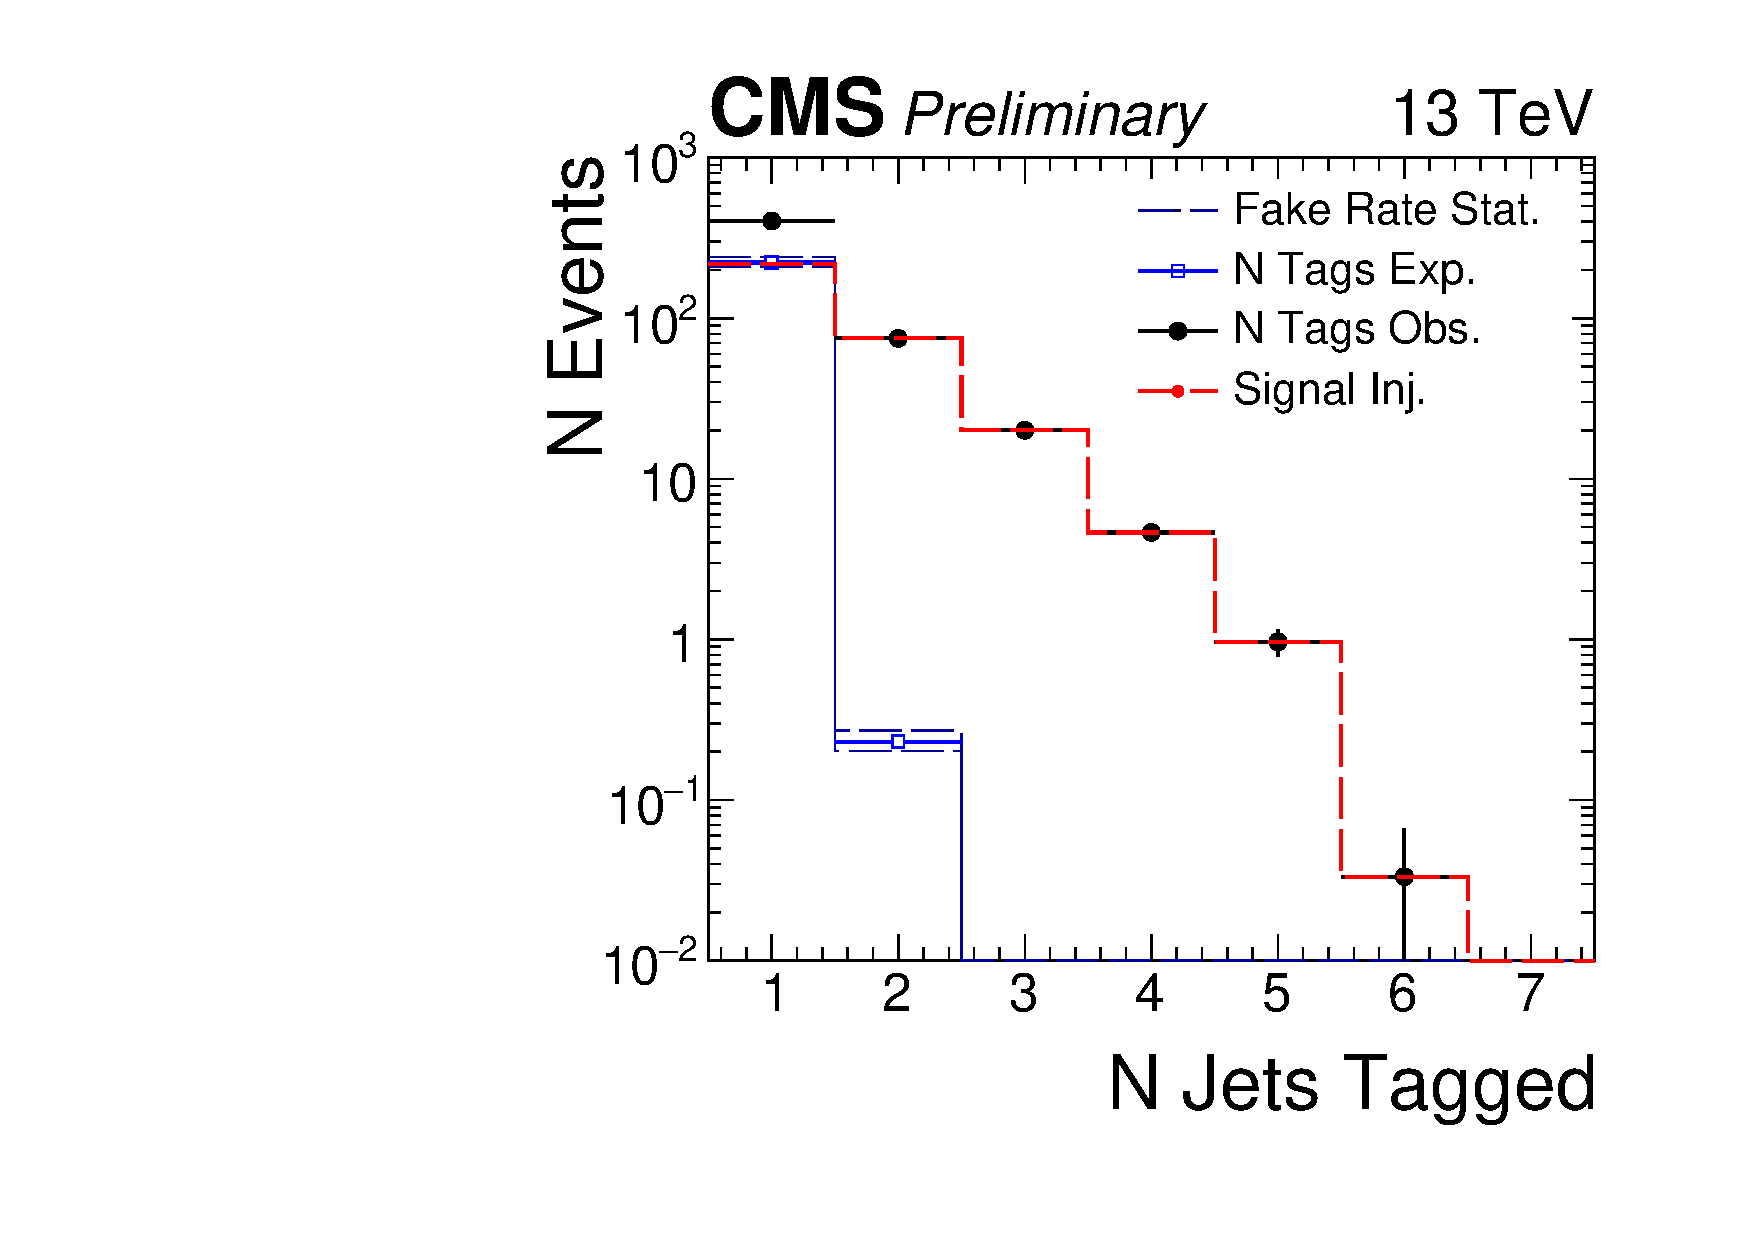
\includegraphics[width=.45\textwidth]{figures/an/ANALYSIS/76x_pu/INJECTION/mx100_ctau10mm_1000ev.pdf}
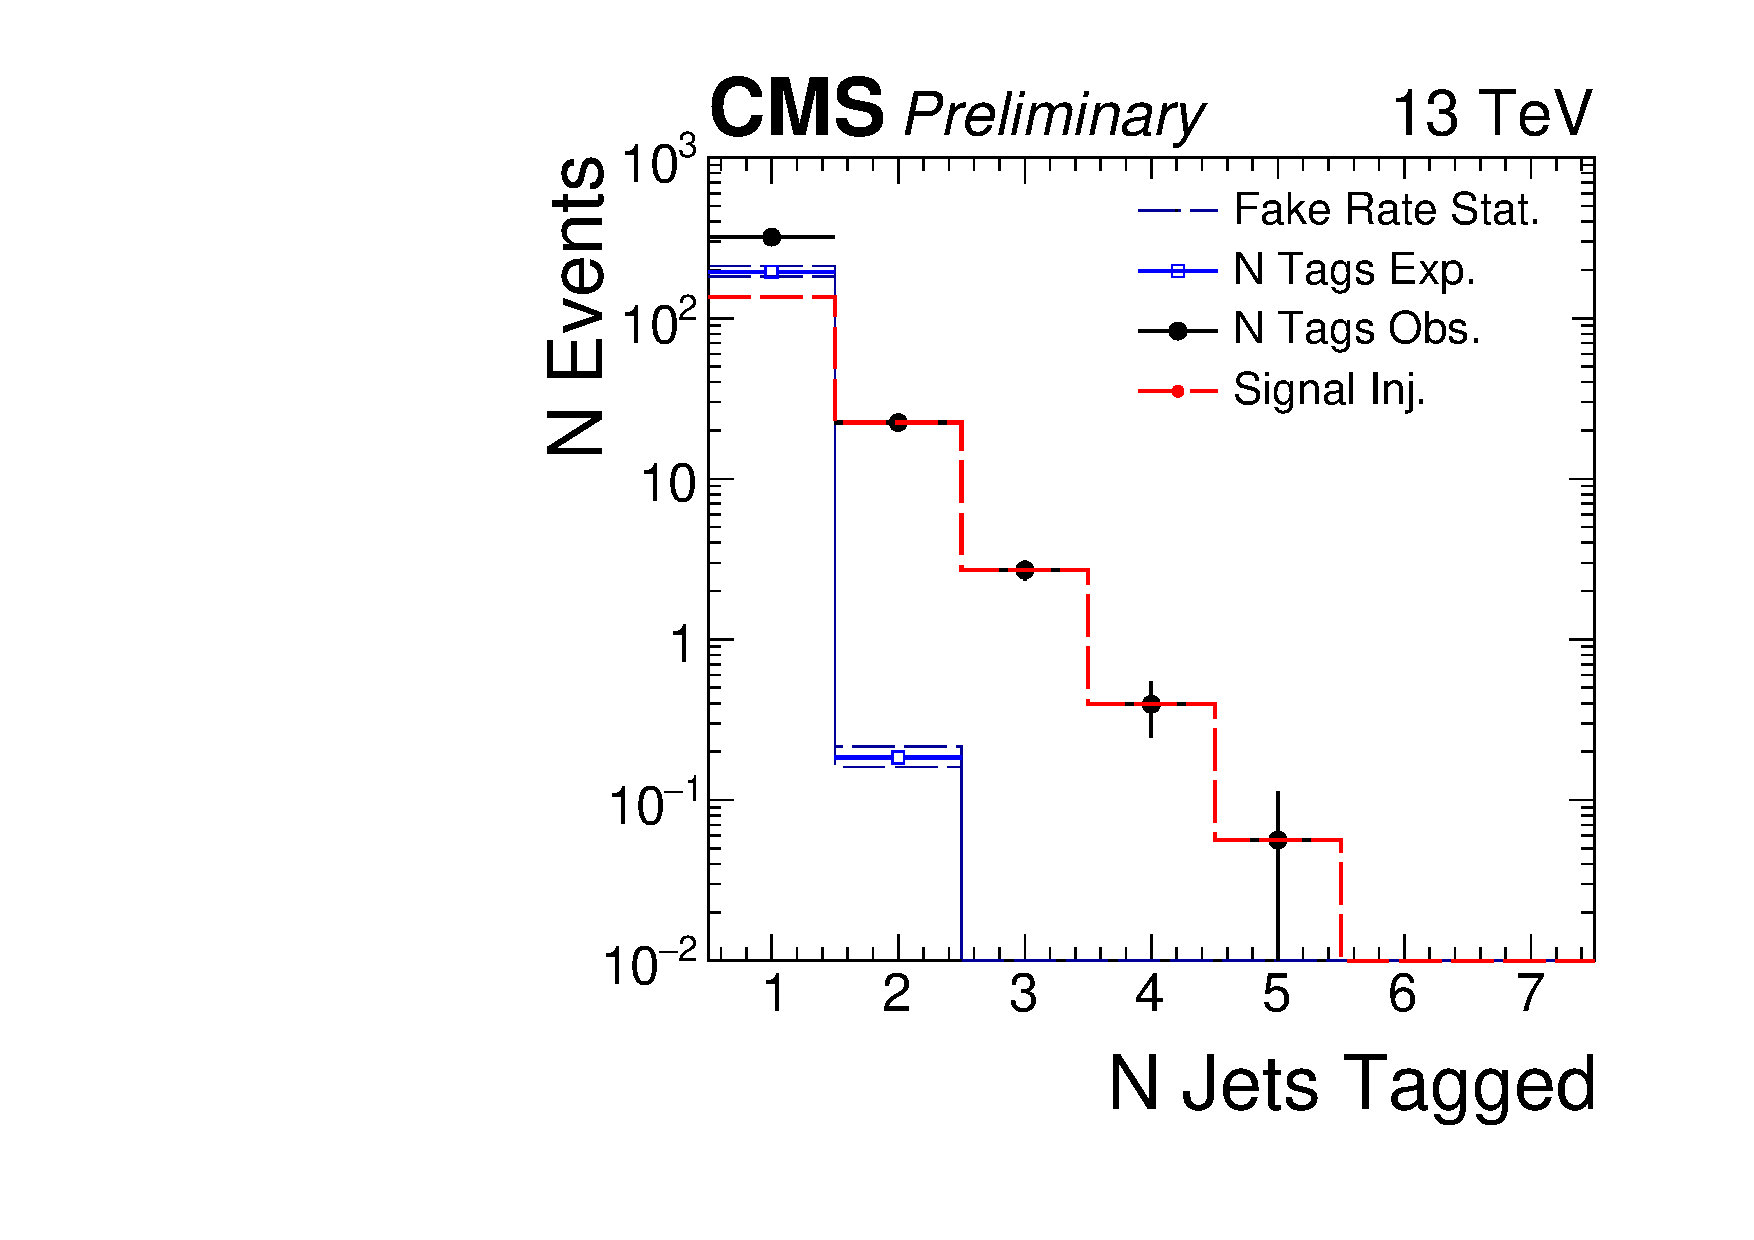
\includegraphics[width=.45\textwidth]{figures/an/ANALYSIS/76x_pu/INJECTION/mx100_ctau1000mm_1000ev.pdf}\\
\caption{Signal Injection. The Jet-Jet signal sample is varied $m_{X^0}=700$~GeV and $c\tau_0=1000$~mm (top left) 
$m_{X^0}=700$ GeV and $c\tau_0=10$~mm (top right) $m_{X^0}=100$ GeV and $c\tau_0=1000$~mm (bottom left) $m_{X^0}=100$~GeV and $c\tau_0=10$~mm (bottom right).
The level of signal contamination is fixed at 100 events for the $m_{X^0}=700$~GeV and 1000 events for $m_{X^0}=100$~GeV. The full 
event selection is applied and the baseline jet tag definition.  
\label{fig:injection_100gev_700gev_100ev}}
\end{center}
\end{figure}

\begin{table}
\caption{The signal injection test using a fixed signal point $m_{{X^0}} = 700$ ~GeV and $c\tau_0 = 10mm$ with varied amount of injection.
 A summary of the 1,2,3, and 4 tag predictions as a function of the number of events injected (top).  The two background systematic errors are
listed separately as $\sigma_{method},\sigma_{fake-rate}$. A summary of the observed number of tags (bottom). 
  \label{tab:700_injection_summary}}
\begin{center}
\begin{tabular}{cccccc}
\hline 
\textbf{Injection} $\sigma\times\mathcal{L}$  & \textbf{1 Pred} & \textbf{2 Pred} & \textbf{3 Pred} &\textbf{4 Pred} \\
\hline
0 &$ 185^{+14,+17}_{-14,-13} $&$0.16^{+0.01,+0.03}_{-0.01,-0.02}$& -- &-- \\
10 &$ 187^{+14,+17}_{-14,-13} $&$0.16^{+0.01,+0.03}_{-0.01,-0.02}$& -- &-- \\
100 &$ 207^{+16,+18}_{-16,-14} $&$0.20^{+0.02,+0.04}_{-0.02,-0.03} $&--&-- \\
1000 &$ 408^{+31,+23}_{-31,-19} $&$0.81^{+0.06,+0.09}_{-0.06,-0.08} $&--&-- \\
10000 &$ 2366^{+177,+53}_{-177,-49} $&$26.95^{+2.02,+1.19}_{-2.02,-1.10} $&$0.18^{+0.01,+0.01}_{-0.01,-0.01} $&-- \\
\hline 
\hline
\textbf{Injection} $\sigma\times\mathcal{L}$ & \textbf{1 Obs} & \textbf{2 Obs} & \textbf{3 Obs} & \textbf{4 Obs}\\
\hline
0 & 185 & -- & -- & -- \\
10 & 187 & 2 & 2 & 1 \\ 
100 & 205 & 23 & 20 & 12 \\
1000 & 386 & 237 & 188 & 116 \\
10000 & 2260 & 2341 & 1976 & 1165 \\
\hline 
\end{tabular} 
\end{center}
\end{table}

\begin{table}
\caption{Signal injection test with fixed number of injected events and varied $c\tau_0$ and $m_{X^0}$. 
A summary of the 1,2,3, and 4 tag predictions as a function of the number of events injected (top). The two background systematic errors are
listed separately as $\sigma_{method},\sigma_{fake-rate}$.  A summary of the observed number of tags (bottom). 
\label{tab:700_100_injection_summary}}
\begin{center}
\begin{tabular}{cccccc}
\hline 
$\sigma\times\mathcal{L}$ & $m_{X^0}$ [GeV] & $c\tau_0$ [mm]  & \textbf{1 Pred} & \textbf{2 Pred} & \textbf{3+4 Pred} \\
\hline
100 &$ 700 $&$ 10 $&$ 207^{+16,+18}_{-16,-14} $&$0.20^{+0.02,+0.04}_{-0.02,-0.03} $&-- \\
100 &$ 700 $&$ 1000 $&$ 202^{+15,+18}_{-15,-14} $&$0.20^{+0.02,+0.03}_{-0.02,-0.03} $&--\\
1000 &$ 100 $&$ 10 $&$222^{+17,+18}_{-17,-14} $&$0.23^{+0.02,+0.04}_{-0.02,-0.03} $&--\\
1000 &$ 100 $&$ 1000 $&$ 195^{+15,+17}_{-15,-13} $&$0.18^{+0.01,+0.03}_{-0.01,-0.02} $&--\\ 
\hline 
\hline 
$\sigma\times\mathcal{L}$ & \textbf{Mass} [GeV] & $c\tau_0$ [mm]  & \textbf{1 Obs} & \textbf{2 Obs} & \textbf{3+4 Obs}  \\
\hline
100 & 700 & 10 & 205 & 23 & 32 \\
100 & 700 & 1000 & 211 & 18 & 12  \\
1000 & 100 & 10 & 404 & 74 & 26 \\
1000 & 100 & 1000 & 321 & 23 & 4  \\
\end{tabular} 
\end{center}
\end{table}

\begin{table}[tb]
  \caption{A summary of the size of the signal injected in the signal injection test (top).
    A summary of signal region yields in the 2,3, and 4 nominal displaced jet tag bins (middle) and  the
    observed number of tags (bottom), as a function of the
    size of the signal contamination, for a signal injection test using a fixed
    signal point $m_{X^0} = 700$ ~GeV and $c\tau_0 = 10$~mm with
    varied signal yields. The no signal case is included as a reference to 
    the predicted values without contamination. The test is normalized such that the sum of signal and background
     events stays fixed at the observed number of events passing the analysis event selection.
    The contamination fraction corresponds to the hypothetical fraction of signal events contained within
     the events passing the event selection.  
    \label{tab:700_injection_summary_norm}}
\begin{center}
\begin{tabular}{cccc}
\textbf{Contam. Fraction} & \textbf{Signal} $\sigma$ [fb] \\ 
\hline
 0 & 0 \\
 0.01\% & 30 \\
 0.10\% & 290 \\
 1.04\% & 3000 \\
 9.47\% & 28000 \\
\end{tabular} 
\begin{tabular}{ccccc}
\textbf{Contamination \%} & \textbf{2 tag pred} & \textbf{3 tag pred} &\textbf{4 tag pred} \\
\hline
 0 &  $1.34^{+0.25}_{-0.17}$ & - & - \\ 
 0.01\% & $1.34^{+0.25}_{-0.17}$ & - & - \\
 0.10\% & $1.67\pm0.33$ & - & - \\
 1.04\% & $6.71^{+0.91}_{-0.82}$ &- & - \\
 9.47\% & $205.38\pm15.21$ & $1.37\pm0.08$ & - \\ 
\\
\textbf{Contamination \%} &  \textbf{2 tag obs} & \textbf{3 tag obs} & \textbf{4 tag obs} \\
\hline
0.00\% & 0 & 0 & 0 \\
0.01\% &  19 & 16 & 10 \\ 
0.10\% &  179 & 159 & 93 \\
1.04\% &  1914 & 1520 & 943   \\
9.47\% &  17632  & 14883 & 8775   \\
\end{tabular} 
\end{center}
\end{table}

To test the response of the background prediction to the presence of signal contamination in the jet probabilities used for the $P(N_{\textrm{tags}})$ derivation,
signal events are `injected` into QCD Monte Carlo. The resulting predictions for varied masses,
lifetimes, and sizes of contamination are shown in Fig. \ref{fig:injection_700_10mm} and Fig. \ref{fig:injection_100gev_700gev_100ev}. The corresponding predictions, observed number of tags, and the
deviation from expectation are summarized in Table \ref{tab:700_injection_summary}
and Table \ref{tab:700_100_injection_summary}. The goal of this exercise
is to understand the quantity of signal contamination, as well as lifetime and mass, required to significantly alter the background prediction. 

The resulting predictions are also reported normalized such that the total number of signal plus QCD events passing the event selection are equal to the number of events passing the
event selection in the analysis in Table \ref{tab:700_injection_summary_norm}.

The change in the $N_{\textrm{tags}}^{\textrm{obs}}$ distribution to the presence of signal is on the order of the number of events with $N_{\textrm{tags}}>2$ whereas 
the integrated shift in $P(N_{\textrm{tags}}\geq2)$ is on the order of the shift induced in the $p(j)$ distribution. This shift is of the order the signal contamination. 
We can conclude the analysis will retain relative sensitivity as long as the signal contamination is relatively smaller than the QCD contribution in 
the fake rate calculation. 

In summary, the background prediction is robust to a variety signal masses, lifetimes and sizes of contamination. In particular, the
background is correctly determined within error in the 0 injection case and the bias to the background prediction due to the 
contamination is small relative to the number of signal events injected.

The following section explores the  sensitivity to signal explicitly in a simplified scenario given the assumption that the jet probabilities accurately predict the
background when there are no signal events present. This assumption is based on the closure studies in the previous section and can be considered
true within some closure systematic.

\subsubsection{Explicit sensitivity in a simplified injection scenario}

Consider a sample of $N_{\textrm{QCD}}$ QCD events with a known fraction of jets that are tagged $f(j_i)$ as a function of some jet parameters $j_i$. 
For simplicity, assume events have exactly 2 jets. Also assume 
we have shown that the observation approximately determined $N_{\textrm{obs}}^{\textrm{2-tag}} = N_{\textrm{pred}}^{\textrm{2-tag}}$ when we interpret $f(j_i)$ as a conditional probability 
$p(j_i)$ such that:
\begin{align*}
N_{\textrm{obs}}^{\textrm{2-tag}} = N_{\textrm{pred}}^{\textrm{2-tag}} = \sum_i [p(j_1)p(j_2)]_{i}  = N_{\textrm{QCD}}p^2 
\end{align*}
where we are using a flat probability $p$ such that  $p(j_1)=p(j_2)=p=n_{\textrm{tag}}/n_{\textrm{jets}} =  n_{\textrm{fake}} / 2N_{\textrm{events}}$. $n_{\textrm{tag}}$ is the number of jets tagged, which in a QCD sample is exactly $n_{\textrm{fake}}$. Now, say we perform the signal injection test by
injecting $N_{\textrm{sig}}$ events with correspondingly $2N_{\textrm{sig}}$ signal jets. Let $\epsilon$ be the efficiency for a signal event to have 1 tag. 
 Accordingly the probability will shift $p(j_i)\rightarrow \tilde{p}(j_i)$:
\begin{align*}
\tilde{p} = \frac{n_{\textrm{fake}} + n_{\textrm{true-tags}}}{2N_{\textrm{QCD}} + 2N_{\textrm{sig}}} = \frac{n_{\textrm{fake}} + \epsilon 2N_{\textrm{sig}} }{2N_{\textrm{QCD}} + 2N_{\textrm{sig}}}
\end{align*}
Expanding in $N_{\textrm{sig}}$ about 0 we obtain:
\begin{align*}
\tilde{p} &= \frac{n_{\textrm{fake}}}{2N_{\textrm{QCD}}} - \frac{N_{\textrm{sig}}n_{\textrm{fake}}}{2(N_{\textrm{QCD}})^2} + \epsilon\frac{2N_{\textrm{sig}} N_{\textrm{QCD}}}{2(N_{\textrm{QCD}})^2}\\
&= p - p\frac{N_{\textrm{sig}}}{N_{\textrm{QCD}}} + \frac{N_{\textrm{sig}}\epsilon}{N_{\textrm{QCD}}}
\end{align*}
Let $\Delta = N_{\textrm{sig}}/{N_{\textrm{QCD}}}$
\begin{align*}
\tilde{p} = p(1-\Delta) + \Delta\epsilon
\end{align*}
Note that as the signal contamination  $\Delta\rightarrow 0$, we obtain the correct probability $\tilde{p}=p$. 
Now we attempt to predict the number of events with 2 tags using $\tilde{p}$ and splitting the sum over signal and QCD events.
\begin{align*}
N_{\textrm{pred}}^{\textrm{2-tag}} &= \sum_i \tilde{p}\tilde{p}\\ 
&= \sum_i (p(1-\Delta) + \Delta\epsilon)^2\\ 
&= \sum_i p^2 - p^2(2\Delta) + p^2\Delta^2 + 2p\Delta \epsilon - 2 p \Delta^2 \epsilon + \Delta^2 \epsilon^2
\end{align*}
We now split the events in the sum between QCD and Signal. 
\begin{align*}
N_{\textrm{pred}}^{\textrm{2-tag}} &= \sum_i (\textrm{QCD}) + \sum_i (\textrm{Signal})\\
\sum_i (\textrm{QCD}) &= N_{\textrm{QCD}} ( p^2 - p^2(2\Delta) + p^2\Delta^2 + 2p\Delta \epsilon - 2 p \Delta^2 \epsilon + \Delta^2 \epsilon^2)\\
&= N_{\textrm{obs}}^{\textrm{QCD}} - N_{\textrm{sig}}(p^2\Delta + \Delta \epsilon^2 - 2p^2 + 2p\epsilon - 2p\Delta \epsilon) 
\end{align*}
where we have used the fact that $\Delta N_{\textrm{QCD}} = N_{\textrm{sig}}$ and $\sum_i p^2 = N_{\textrm{obs}}^{\textrm{QCD}}$:
\begin{align*}
\sum_i(\textrm{Signal}) =  N_{\textrm{sig}}(  p^2 - p^2(2\Delta) + p^2\Delta^2 + 2p\Delta \epsilon - 2 p \Delta^2 \epsilon + \Delta^2 \epsilon^2)
\end{align*}
We now evaluate the disagreement between observed and prediction by the variable $S$. Let 
$N_{\textrm{obs}}^{\textrm{2-tag}} = N_{\textrm{obs}}^{\textrm{sig}} + N_{\textrm{obs}}^{\textrm{QCD}}$. The sensitivity $S$, is a measure of how well we have predicted the background
in the presence of signal. When $S=1$ the prediction is exactly the background and the excess is exactly the number of signal events. 
When $S=0$ the probabilities prediction has over estimated the background entirely resulting in no disagreement between observed and predicted 
2 tag events.
\begin{align*}
S = \frac{N_{\textrm{obs}}^{\textrm{2-tag}} - N_{\textrm{pred}}^{\textrm{2-tag}} }{N_{\textrm{sig}}} = 1 &- (2p\epsilon + \Delta \epsilon^2) \\
&- (p^2 + \Delta^2\epsilon^2 +  2p\Delta\epsilon -2p^2  - 2p\Delta\epsilon) \\
&- (p^2\Delta -2p^2\Delta -2p\Delta^2\epsilon) \\
&- (p^2\Delta^2)
\end{align*}
Terms are grouped by their order in $O(\Delta)+O(p)$. Consider the case when $\epsilon \approx 1$ (this is an approximation for readability as $\epsilon=1$ would imply no 2 tag events) and for simplicity say $\Delta = p = x$.
\begin{align*}
S= 1 - 3x + 3 x^3 - x^4
\end{align*}
The analysis sensitivity to signal as a fraction of the signal present is 
at leading order $1-3x$. As the misidentification rate in the analysis is small $O(10^{-4})$,  we conclude signal contamination will negligibly affect the sensitivity of the analysis. 

